% Generated by Sphinx.
\documentclass[letterpaper,10pt,english]{manual}
\usepackage[utf8]{inputenc}
\usepackage[T1]{fontenc}
\usepackage{babel}
\usepackage{times}
\usepackage[Bjarne]{fncychap}
\usepackage{longtable}
\usepackage{sphinx}


\title{Django Stories Documentation}
\date{April 20, 2010}
\release{0.2}
\author{The Washington Times}
\newcommand{\sphinxlogo}{}
\renewcommand{\releasename}{Release}
\makeindex
\makemodindex

\makeatletter
\def\PYG@reset{\let\PYG@it=\relax \let\PYG@bf=\relax%
    \let\PYG@ul=\relax \let\PYG@tc=\relax%
    \let\PYG@bc=\relax \let\PYG@ff=\relax}
\def\PYG@tok#1{\csname PYG@tok@#1\endcsname}
\def\PYG@toks#1+{\ifx\relax#1\empty\else%
    \PYG@tok{#1}\expandafter\PYG@toks\fi}
\def\PYG@do#1{\PYG@bc{\PYG@tc{\PYG@ul{%
    \PYG@it{\PYG@bf{\PYG@ff{#1}}}}}}}
\def\PYG#1#2{\PYG@reset\PYG@toks#1+\relax+\PYG@do{#2}}

\def\PYG@tok@gd{\def\PYG@tc##1{\textcolor[rgb]{0.63,0.00,0.00}{##1}}}
\def\PYG@tok@gu{\let\PYG@bf=\textbf\def\PYG@tc##1{\textcolor[rgb]{0.50,0.00,0.50}{##1}}}
\def\PYG@tok@gt{\def\PYG@tc##1{\textcolor[rgb]{0.00,0.25,0.82}{##1}}}
\def\PYG@tok@gs{\let\PYG@bf=\textbf}
\def\PYG@tok@gr{\def\PYG@tc##1{\textcolor[rgb]{1.00,0.00,0.00}{##1}}}
\def\PYG@tok@cm{\let\PYG@it=\textit\def\PYG@tc##1{\textcolor[rgb]{0.25,0.50,0.56}{##1}}}
\def\PYG@tok@vg{\def\PYG@tc##1{\textcolor[rgb]{0.73,0.38,0.84}{##1}}}
\def\PYG@tok@m{\def\PYG@tc##1{\textcolor[rgb]{0.13,0.50,0.31}{##1}}}
\def\PYG@tok@mh{\def\PYG@tc##1{\textcolor[rgb]{0.13,0.50,0.31}{##1}}}
\def\PYG@tok@cs{\def\PYG@tc##1{\textcolor[rgb]{0.25,0.50,0.56}{##1}}\def\PYG@bc##1{\colorbox[rgb]{1.00,0.94,0.94}{##1}}}
\def\PYG@tok@ge{\let\PYG@it=\textit}
\def\PYG@tok@vc{\def\PYG@tc##1{\textcolor[rgb]{0.73,0.38,0.84}{##1}}}
\def\PYG@tok@il{\def\PYG@tc##1{\textcolor[rgb]{0.13,0.50,0.31}{##1}}}
\def\PYG@tok@go{\def\PYG@tc##1{\textcolor[rgb]{0.19,0.19,0.19}{##1}}}
\def\PYG@tok@cp{\def\PYG@tc##1{\textcolor[rgb]{0.00,0.44,0.13}{##1}}}
\def\PYG@tok@gi{\def\PYG@tc##1{\textcolor[rgb]{0.00,0.63,0.00}{##1}}}
\def\PYG@tok@gh{\let\PYG@bf=\textbf\def\PYG@tc##1{\textcolor[rgb]{0.00,0.00,0.50}{##1}}}
\def\PYG@tok@ni{\let\PYG@bf=\textbf\def\PYG@tc##1{\textcolor[rgb]{0.84,0.33,0.22}{##1}}}
\def\PYG@tok@nl{\let\PYG@bf=\textbf\def\PYG@tc##1{\textcolor[rgb]{0.00,0.13,0.44}{##1}}}
\def\PYG@tok@nn{\let\PYG@bf=\textbf\def\PYG@tc##1{\textcolor[rgb]{0.05,0.52,0.71}{##1}}}
\def\PYG@tok@no{\def\PYG@tc##1{\textcolor[rgb]{0.38,0.68,0.84}{##1}}}
\def\PYG@tok@na{\def\PYG@tc##1{\textcolor[rgb]{0.25,0.44,0.63}{##1}}}
\def\PYG@tok@nb{\def\PYG@tc##1{\textcolor[rgb]{0.00,0.44,0.13}{##1}}}
\def\PYG@tok@nc{\let\PYG@bf=\textbf\def\PYG@tc##1{\textcolor[rgb]{0.05,0.52,0.71}{##1}}}
\def\PYG@tok@nd{\let\PYG@bf=\textbf\def\PYG@tc##1{\textcolor[rgb]{0.33,0.33,0.33}{##1}}}
\def\PYG@tok@ne{\def\PYG@tc##1{\textcolor[rgb]{0.00,0.44,0.13}{##1}}}
\def\PYG@tok@nf{\def\PYG@tc##1{\textcolor[rgb]{0.02,0.16,0.49}{##1}}}
\def\PYG@tok@si{\let\PYG@it=\textit\def\PYG@tc##1{\textcolor[rgb]{0.44,0.63,0.82}{##1}}}
\def\PYG@tok@s2{\def\PYG@tc##1{\textcolor[rgb]{0.25,0.44,0.63}{##1}}}
\def\PYG@tok@vi{\def\PYG@tc##1{\textcolor[rgb]{0.73,0.38,0.84}{##1}}}
\def\PYG@tok@nt{\let\PYG@bf=\textbf\def\PYG@tc##1{\textcolor[rgb]{0.02,0.16,0.45}{##1}}}
\def\PYG@tok@nv{\def\PYG@tc##1{\textcolor[rgb]{0.73,0.38,0.84}{##1}}}
\def\PYG@tok@s1{\def\PYG@tc##1{\textcolor[rgb]{0.25,0.44,0.63}{##1}}}
\def\PYG@tok@gp{\let\PYG@bf=\textbf\def\PYG@tc##1{\textcolor[rgb]{0.78,0.36,0.04}{##1}}}
\def\PYG@tok@sh{\def\PYG@tc##1{\textcolor[rgb]{0.25,0.44,0.63}{##1}}}
\def\PYG@tok@ow{\let\PYG@bf=\textbf\def\PYG@tc##1{\textcolor[rgb]{0.00,0.44,0.13}{##1}}}
\def\PYG@tok@sx{\def\PYG@tc##1{\textcolor[rgb]{0.78,0.36,0.04}{##1}}}
\def\PYG@tok@bp{\def\PYG@tc##1{\textcolor[rgb]{0.00,0.44,0.13}{##1}}}
\def\PYG@tok@c1{\let\PYG@it=\textit\def\PYG@tc##1{\textcolor[rgb]{0.25,0.50,0.56}{##1}}}
\def\PYG@tok@kc{\let\PYG@bf=\textbf\def\PYG@tc##1{\textcolor[rgb]{0.00,0.44,0.13}{##1}}}
\def\PYG@tok@c{\let\PYG@it=\textit\def\PYG@tc##1{\textcolor[rgb]{0.25,0.50,0.56}{##1}}}
\def\PYG@tok@mf{\def\PYG@tc##1{\textcolor[rgb]{0.13,0.50,0.31}{##1}}}
\def\PYG@tok@err{\def\PYG@bc##1{\fcolorbox[rgb]{1.00,0.00,0.00}{1,1,1}{##1}}}
\def\PYG@tok@kd{\let\PYG@bf=\textbf\def\PYG@tc##1{\textcolor[rgb]{0.00,0.44,0.13}{##1}}}
\def\PYG@tok@ss{\def\PYG@tc##1{\textcolor[rgb]{0.32,0.47,0.09}{##1}}}
\def\PYG@tok@sr{\def\PYG@tc##1{\textcolor[rgb]{0.14,0.33,0.53}{##1}}}
\def\PYG@tok@mo{\def\PYG@tc##1{\textcolor[rgb]{0.13,0.50,0.31}{##1}}}
\def\PYG@tok@mi{\def\PYG@tc##1{\textcolor[rgb]{0.13,0.50,0.31}{##1}}}
\def\PYG@tok@kn{\let\PYG@bf=\textbf\def\PYG@tc##1{\textcolor[rgb]{0.00,0.44,0.13}{##1}}}
\def\PYG@tok@o{\def\PYG@tc##1{\textcolor[rgb]{0.40,0.40,0.40}{##1}}}
\def\PYG@tok@kr{\let\PYG@bf=\textbf\def\PYG@tc##1{\textcolor[rgb]{0.00,0.44,0.13}{##1}}}
\def\PYG@tok@s{\def\PYG@tc##1{\textcolor[rgb]{0.25,0.44,0.63}{##1}}}
\def\PYG@tok@kp{\def\PYG@tc##1{\textcolor[rgb]{0.00,0.44,0.13}{##1}}}
\def\PYG@tok@w{\def\PYG@tc##1{\textcolor[rgb]{0.73,0.73,0.73}{##1}}}
\def\PYG@tok@kt{\def\PYG@tc##1{\textcolor[rgb]{0.56,0.13,0.00}{##1}}}
\def\PYG@tok@sc{\def\PYG@tc##1{\textcolor[rgb]{0.25,0.44,0.63}{##1}}}
\def\PYG@tok@sb{\def\PYG@tc##1{\textcolor[rgb]{0.25,0.44,0.63}{##1}}}
\def\PYG@tok@k{\let\PYG@bf=\textbf\def\PYG@tc##1{\textcolor[rgb]{0.00,0.44,0.13}{##1}}}
\def\PYG@tok@se{\let\PYG@bf=\textbf\def\PYG@tc##1{\textcolor[rgb]{0.25,0.44,0.63}{##1}}}
\def\PYG@tok@sd{\let\PYG@it=\textit\def\PYG@tc##1{\textcolor[rgb]{0.25,0.44,0.63}{##1}}}

\def\PYGZat{@}
\def\PYGZlb{[}
\def\PYGZrb{]}
\makeatother

\begin{document}

\maketitle
\tableofcontents
\hypertarget{--doc-index}{}


Contents:

\resetcurrentobjects
\hypertarget{--doc-install}{}

\chapter{Installation}

\#\#\# * Add javascript for advanced and simple modes of editing \#\#\# Maybe not
\begin{itemize}
\item {} 
Move authors to own section and below content.

\item {} 
Auto-add the user if it is a new story

\item {} 
Remove pluggable markups from settings and models

\item {} 
Super Users can see everything!

\item {} 
new templates for reversion to make it not editable, and show changes (optionally?)

\end{itemize}

Dependencies:
\begin{quote}

diff\_match\_patch (included in lib)
\end{quote}

Integration with django-tinymce

Integration with django-reversion

Integration with django-categories

\resetcurrentobjects
\hypertarget{--doc-settings}{}

\hypertarget{settings}{}\chapter{Settings}

Here are several settings that you can use to customize Stories.


\hypertarget{story-status-choices}{}\section{STORY\_STATUS\_CHOICES}

A story can be in several different states, for example draft vs. live. Your workflow might have several states that a story goes through, but there can only be one choice that is considered ``Published''.

Choices are specified as a \code{list} or \code{tuple} of \code{integer} - \code{string} tuples. The \code{integer} is the code for the choice and the \code{string} is the description that the user sees.

\textbf{Defaults:}

\begin{Verbatim}[commandchars=@\[\]]
@PYG[n][STORY@_STATUS@_CHOICES] @PYG[o][=] @PYG[p][(]
    @PYG[p][(]@PYG[l+m+mi][1]@PYG[p][,] @PYG[l+s][']@PYG[l+s][DRAFT]@PYG[l+s][']@PYG[p][)]@PYG[p][,]
    @PYG[p][(]@PYG[l+m+mi][2]@PYG[p][,] @PYG[l+s][']@PYG[l+s][READY FOR EDITING]@PYG[l+s][']@PYG[p][)]@PYG[p][,]
    @PYG[p][(]@PYG[l+m+mi][3]@PYG[p][,] @PYG[l+s][']@PYG[l+s][READY TO PUBLISH]@PYG[l+s][']@PYG[p][)]@PYG[p][,]
    @PYG[p][(]@PYG[l+m+mi][4]@PYG[p][,] @PYG[l+s][']@PYG[l+s][PUBLISHED]@PYG[l+s][']@PYG[p][)]@PYG[p][,]
    @PYG[p][(]@PYG[l+m+mi][5]@PYG[p][,] @PYG[l+s][']@PYG[l+s][REJECTED]@PYG[l+s][']@PYG[p][)]@PYG[p][,]
    @PYG[p][(]@PYG[l+m+mi][6]@PYG[p][,] @PYG[l+s][']@PYG[l+s][UN-PUBLISHED]@PYG[l+s][']@PYG[p][)]@PYG[p][,]
@PYG[p][)]
\end{Verbatim}

\emph{Draft:} A work-in-progress.

\emph{Ready for Editing:} The story is ready for an editor's touch.

\emph{Ready to Publish:} The editing is finished and the story is ready to go on to the web site.

\emph{Published:} The story is on the web site, as long as it is past the story's publish date and time.

\emph{Rejected:} The editor didn't like something and the author needs to work on it some more.

\emph{Un-published:} The story has been removed from the site for some reason.
\hypertarget{story-default-status}{}

\section{STORY\_DEFAULT\_STATUS}

When a story is created, what should the the status default to?

\textbf{Default:}

\begin{Verbatim}[commandchars=@\[\]]
@PYG[n][STORY@_DEFAULT@_STATUS] @PYG[o][=] @PYG[l+m+mi][1] @PYG[c][@# Draft]
\end{Verbatim}
\hypertarget{story-published-status}{}

\section{STORY\_PUBLISHED\_STATUS}

Which one of the possible statuses is considered ``On Site.''

\textbf{Default:}

\begin{Verbatim}[commandchars=@\[\]]
@PYG[n][STORY@_PUBLISHED@_STATUS] @PYG[o][=] @PYG[l+m+mi][4] @PYG[c][@# Published]
\end{Verbatim}
\hypertarget{story-origin-choices}{}

\section{STORY\_ORIGIN\_CHOICES}

It is possible that stories could be coming in from several sources, such as a wire service, an editorial front end, or an FTP site. This settings allows you to mark which stories originated from which source, so you can potentially do something different depending on the source. For example, include all stories in the RSS feed, except ones that came from a wire service.

Choices are specified as a \code{list} or \code{tuple} of \code{integer} - \code{string} tuples. The \code{integer} is the code for the choice and the \code{string} is the description that the user sees.

\textbf{Default:}

\begin{Verbatim}[commandchars=@\[\]]
@PYG[n][STORY@_ORIGIN@_CHOICES] @PYG[o][=] @PYG[p][(]
    @PYG[p][(]@PYG[l+m+mi][0]@PYG[p][,] @PYG[l+s][']@PYG[l+s][Admin]@PYG[l+s][']@PYG[p][)]@PYG[p][,]
@PYG[p][)]
\end{Verbatim}
\hypertarget{story-default-origin}{}

\section{STORY\_DEFAULT\_ORIGIN}

When a story is created from the Django Admin, which choice of origin should it default to?

\textbf{Default:}

\begin{Verbatim}[commandchars=@\[\]]
@PYG[n][STORY@_DEFAULT@_ORIGIN] @PYG[o][=] @PYG[l+m+mi][0] @PYG[c][@# Admin]
\end{Verbatim}
\hypertarget{story-include-print}{}

\section{STORY\_INCLUDE\_PRINT}

Should the fields related to print production be included in the database. The fields are \code{print\_pub\_date}, \code{print\_section}, and \code{print\_page}.

\textbf{Default:}

\begin{Verbatim}[commandchars=@\[\]]
@PYG[n][STORY@_INCLUDE@_PRINT] @PYG[o][=] @PYG[n+nb+bp][False]
\end{Verbatim}
\hypertarget{story-relation-models}{}

\section{STORY\_RELATION\_MODELS}

A story can relate to several other things, such as other stories, photographs, photo galleries, and external links. Stories links to the Django Content Types application, which would normally show all sorts of things that don't matter to the author and end users. This setting specifies which specific models are relatable to a story.

The value should be a tuple of \emph{`appname.modelname'} strings.

If this setting is empty or \code{None}, the story relations are not available in the admin. If at a later time you decide to set this, you must \code{syncdb} before it will work properly.

\textbf{Default:}

\begin{Verbatim}[commandchars=@\[\]]
@PYG[n][STORY@_RELATION@_MODELS] @PYG[o][=] @PYG[n+nb+bp][None] @PYG[c][@# Not enabled]
\end{Verbatim}
\hypertarget{story-pagination}{}

\section{STORY\_PAGINATION}

Django Stories has a built-in \code{Paginator} subclass that splits HTML-formatted text into paragraphs for paginating. If \code{STORY\_PAGINATION} is \code{True}, stories will be paginated in the template. See \hyperlink{pagination}{\emph{Pagination}} for more information, and the
\href{http://docs.djangoproject.com/en/dev/topics/pagination/\#paginator-objects}{Django Paginator docs} for more about pagination is general.

\textbf{Default:}

\begin{Verbatim}[commandchars=@\[\]]
@PYG[n][STORY@_PAGINATION] @PYG[o][=] @PYG[n+nb+bp][False]
\end{Verbatim}
\hypertarget{story-p-per-page}{}

\section{STORY\_P\_PER\_PAGE}

If \code{STORY\_PAGINATION} is \code{True}, then this setting sets the number of paragraphs per page for pagination.

\textbf{Default:}

\begin{Verbatim}[commandchars=@\[\]]
@PYG[n][STORY@_P@_PER@_PAGE] @PYG[o][=] @PYG[l+m+mi][20]
\end{Verbatim}
\hypertarget{story-orphans}{}

\section{STORY\_ORPHANS}

If \code{STORY\_PAGINATION} is \code{True}, then this setting sets the minimum number of paragraphs allowed on the last page for pagination. This means that with \code{STORY\_P\_PER\_PAGE = 20} and \code{STORY\_ORPHANS = 4} a story with 24 paragraphs would only have one page, but a story with 25 paragraphs would have two pages.

\textbf{Default:}

\begin{Verbatim}[commandchars=@\[\]]
@PYG[n][STORY@_ORPHANS] @PYG[o][=] @PYG[l+m+mi][4]
\end{Verbatim}

\resetcurrentobjects
\hypertarget{--doc-pagination}{}

\hypertarget{pagination}{}\chapter{Pagination}

Many sites wish to paginate long stories over multiple pages. Paginating text is a bit different from paginating a list of objects. Django Stories has a \code{Paginator} subclass that takes an HTML-formatted string instead of a \code{QuerySet}.

The simplest way to use pagination with stories is to set \hyperlink{story-pagination}{\emph{STORY\_PAGINATION}} to \code{True}, which changes the view that handles the story rendering.


\section{Settings that affect pagination}
\begin{description}
\item[\hyperlink{story-pagination}{\emph{STORY\_PAGINATION}}] \leavevmode
Enables or disables pagination altogether. It is disabled by default.

\item[\hyperlink{story-p-per-page}{\emph{STORY\_P\_PER\_PAGE}}] \leavevmode
The number of paragraphs to show on each page. It shows 20 paragraphs by default, but only if story pagination is enabled.

\item[\hyperlink{story-orphans}{\emph{STORY\_ORPHANS}}] \leavevmode
The minimum number of paragraphs allowed allowed on the last page. It is set to 4 by default (meaning a minimum of 5 paragraphs on a page), but only if story pagination is enabled.

\end{description}


\section{Using pagination in templates}

The default name of the story template is \code{stories/pag\_story.html}. Within the context there are two variables:
\begin{description}
\item[story] \leavevmode
The \code{Story} object.

\item[story\_content] \leavevmode
The \code{ParagraphPaginator} class. It contains all the paragraphs of the \code{Story} that should be on this page. A detailed reference of all the methods is in the \href{http://docs.djangoproject.com/en/dev/topics/pagination/\#paginator-objects}{Django Paginator docs}.

\end{description}


\subsection{Different heading on first page}

\begin{Verbatim}[commandchars=@\[\]]
{@% if story@_content.has@_previous @%}
        @textless[]h3@textgreater[]{{ story.headline }}@textless[]/h3@textgreater[]
        @textless[]p@textgreater[]@textless[]em@textgreater[]continued from page {{ story@_content.previous@_page@_number }}@textless[]/em@textgreater[]@textless[]/p@textgreater[]
{@% else @%}
        @textless[]h1@textgreater[]{{ story.headline }}@textless[]/h1@textgreater[]
        @textless[]h2@textgreater[]{{ story.subheadline }}@textless[]/h2@textgreater[]
{@% endif @%}
\end{Verbatim}

The above template snippet checks to see if this is a page other than 1 (meaning it has a previous page) and displays a small headline with a ``continued from page x'' below it.

If it is the first page, it displays the headline and subheadline in all their glory.


\subsection{Looping through the paragraphs}

\begin{Verbatim}[commandchars=@\[\]]
{@% load add@_attribute @%}
{@% for paragraph in story@_content.object@_list @%}
        {@% ifequal story@_content.number 1 @%}
                {@% if forloop.first @%}
                        {{ paragraph@textbar[]add@_attribute:"class=dropcap"@textbar[]safe }}
                {@% else @%}
                        {{ paragraph@textbar[]safe }}
                        {@% endif @%}
        {@% endifequal @%}
{@% endfor @%}
\end{Verbatim}

\code{add\_attribute} is a filter that is included in Django Stories. It adds any attribute to the paragraph. In this example, it checks if it is the first paragraph and adds the attribute \code{class} with a value of \code{dropcap} to the \code{\textless{}p\textgreater{}} tag. That part is unnecessary, but allows you some artistic freedom.

Don't forget the \code{\textbar{}safe} filter at the end. Django will automatically escape all the tags otherwise.


\subsection{Leading them to the next page}

\begin{Verbatim}[commandchars=@\[\]]
{@% if story@_content.has@_next @%}
        @textless[]p@textgreater[]@textless[]a href="?page={{ story@_content.next@_page@_number }}"@textgreater[]@textless[]em@textgreater[]Story Continues @&rarr;@textless[]/em@textgreater[]@textless[]/a@textgreater[]
{@% endif @%}
\end{Verbatim}

Before we hit the typical pagination anchors, it can be nice to add a simple link to the next page, so the reader doesn't have to think about which button to click.


\subsection{The pagination widget}

Django stories includes a template to show a list of pages with previous and next buttons. The template is in \code{stories/pagination\_widget.html} and you can override it should you wish or simple include some styles in your CSS. Add the following line in your template:

\begin{Verbatim}[commandchars=@\[\]]
{@% include "stories/pagination@_widget.html" @%}
\end{Verbatim}

and it will generate some HTML similar to:

\begin{Verbatim}[commandchars=@\[\]]
@textless[]div class="pagination"@textgreater[]
        @textless[]a href="?page=1" class="previous"@textgreater[]@&larr; Previous@textless[]/a@textgreater[]
        @textless[]a href="?page=1" class="page"@textgreater[]1@textless[]/a@textgreater[]
        @textless[]span class="current"@textgreater[]2@textless[]/span@textgreater[]
        @textless[]a href="?page=3" class="page"@textgreater[]3@textless[]/a@textgreater[]
        @textless[]a href="?page=3" class="next"@textgreater[]Next @&rarr;@textless[]/a@textgreater[]
@textless[]/div@textgreater[]
\end{Verbatim}


\subsection{Pagination widget CSS styles}
\begin{description}
\item[\code{div.pagination}] \leavevmode
The wrapper around the entire widget

\item[\code{div.pagination a.previous}] \leavevmode
The anchor for the ``previous'' link

\item[\code{div.pagination a.page}] \leavevmode
The anchor for each page link

\item[\code{div.pagination span.current}] \leavevmode
The wrapper for the current page number

\item[\code{div.pagination a.next}] \leavevmode
The anchor for the ``next'' link

\end{description}

\resetcurrentobjects
\hypertarget{--doc-integration/index}{}

\hypertarget{integration-index}{}\chapter{Integration with Other Django Applications}

\resetcurrentobjects
\hypertarget{--doc-integration/reversion_integration}{}

\hypertarget{reversion-integration}{}\section{Integrating with Django Reversion}
\begin{enumerate}
\item {} 
Install \href{http://code.google.com/p/django-reversion/}{django-reversion}

\begin{Verbatim}[commandchars=@\[\]]
pip install django-reversion
\end{Verbatim}

\item {} 
Add \code{reversion} to your \code{INSTALLED\_APPS} setting.

\item {} 
\code{./manage.py syncdb}

\end{enumerate}

All the hooks are there to notice when reversion is installed. Versions are tracked from when reversion is first installed.

\resetcurrentobjects
\hypertarget{--doc-integration/tinymce_integration}{}

\hypertarget{tinymce-integration}{}\section{Integrating with Django TinyMCE}


\subsection{Install django-tinymce}

Django-tinymce makes it very easy to include a GUI text editor for any textarea.
\begin{enumerate}
\item {} 
Install a special fork of \href{http://code.google.com/p/django-tinymce/}{django-tinymce}  from \href{http://github.com/justquick/django-tinymce}{github}

\begin{Verbatim}[commandchars=@\[\]]
pip install git+http://github.com/justquick/django-tinymce.git@#egg=tinymce
\end{Verbatim}

\item {} 
Download \href{http://tinymce.moxiecode.com/download.php}{TinyMCE} and copy the contents of the \code{jscript} directory into a \code{js} directory within your \code{MEDIA\_ROOT} directory.

\begin{Verbatim}[commandchars=@\[\]]
/myproject
    /apps
    /static
        /css
        /img
        /js
--------@textgreater[]   /tinymce
\end{Verbatim}

\item {} 
Add \code{tinymce} to your \code{INSTALLED\_APPS} setting.

\begin{Verbatim}[commandchars=@\[\]]
INSTALLED@_APPS = (
    ...
    'tinymce',
)
\end{Verbatim}

\item {} 
Add \code{(r'\textasciicircum{}tinymce/', include('tinymce.urls')),} to your \code{urls.py}.

\begin{Verbatim}[commandchars=@\[\]]
@PYG[n][urlpatterns] @PYG[o][=] @PYG[n][patterns]@PYG[p][(]@PYG[l+s][']@PYG[l+s][']@PYG[p][,]
    @PYG[o][.]@PYG[o][.]@PYG[o][.]
    @PYG[p][(]@PYG[l+s][r']@PYG[l+s][@textasciicircum[]tinymce/]@PYG[l+s][']@PYG[p][,] @PYG[n][include]@PYG[p][(]@PYG[l+s][']@PYG[l+s][tinymce.urls]@PYG[l+s][']@PYG[p][)]@PYG[p][)]@PYG[p][,]
    @PYG[o][.]@PYG[o][.]@PYG[o][.]
@PYG[p][)]
\end{Verbatim}

\item {} 
Add the settings for tinymce. The configuration of plugins and tools shown here is just an example. See the \href{http://github.com/justquick/django-tinymce/blob/master/docs/installation.rst}{django-tinymce docs} and \href{http://wiki.moxiecode.com/index.php/TinyMCE:Configuration}{TinyMCE Manual} for more information. For example:

\begin{Verbatim}[commandchars=@\[\]]
@PYG[n][TINYMCE@_DEFAULT@_CONFIG] @PYG[o][=] @PYG[p][{]
    @PYG[l+s][']@PYG[l+s][theme]@PYG[l+s][']@PYG[p][:] @PYG[l+s]["]@PYG[l+s][advanced]@PYG[l+s]["]@PYG[p][,]
    @PYG[l+s][']@PYG[l+s][relative@_urls]@PYG[l+s][']@PYG[p][:] @PYG[n+nb+bp][False]@PYG[p][,]
    @PYG[l+s][']@PYG[l+s][plugins]@PYG[l+s][']@PYG[p][:] @PYG[l+s]["]@PYG[l+s][safari,paste,advimage,preview]@PYG[l+s]["]@PYG[p][,]
    @PYG[l+s][']@PYG[l+s][theme@_advanced@_toolbar@_location]@PYG[l+s]['] @PYG[p][:] @PYG[l+s]["]@PYG[l+s][top]@PYG[l+s]["]@PYG[p][,]
    @PYG[l+s][']@PYG[l+s][theme@_advanced@_toolbar@_align]@PYG[l+s]['] @PYG[p][:] @PYG[l+s]["]@PYG[l+s][left]@PYG[l+s]["]@PYG[p][,]
    @PYG[l+s][']@PYG[l+s][theme@_advanced@_buttons1]@PYG[l+s]['] @PYG[p][:] @PYG[l+s]["]@PYG[l+s][formatselect,bold,italic,underline,separator,bullist,numlist,separator,undo,separator,link,unlink,separator,charmap,image,paste,pasteword,separator,code,preview]@PYG[l+s]["]@PYG[p][,]
    @PYG[l+s][']@PYG[l+s][theme@_advanced@_buttons2]@PYG[l+s]['] @PYG[p][:] @PYG[l+s]["]@PYG[l+s]["]@PYG[p][,]
    @PYG[l+s][']@PYG[l+s][theme@_advanced@_buttons3]@PYG[l+s]['] @PYG[p][:] @PYG[l+s]["]@PYG[l+s]["]@PYG[p][,]
    @PYG[c][@#'skin': 'thebigreason',]
        @PYG[l+s][']@PYG[l+s][theme@_advanced@_statusbar@_location]@PYG[l+s]['] @PYG[p][:] @PYG[l+s]["]@PYG[l+s][bottom]@PYG[l+s]["]@PYG[p][,]
        @PYG[l+s][']@PYG[l+s][width]@PYG[l+s][']@PYG[p][:] @PYG[l+s]["]@PYG[l+s][600]@PYG[l+s]["]@PYG[p][,]
        @PYG[l+s][']@PYG[l+s][height]@PYG[l+s][']@PYG[p][:] @PYG[l+s]["]@PYG[l+s][600]@PYG[l+s]["]@PYG[p][,]
@PYG[p][}]
\end{Verbatim}

\item {} 
Add the \code{TINYMCE\_ADMIN\_FIELDS} setting:

\begin{Verbatim}[commandchars=@\[\]]
@PYG[n][TINYMCE@_ADMIN@_FIELDS] @PYG[o][=] @PYG[p][{]
    @PYG[l+s][']@PYG[l+s][stories.story]@PYG[l+s][']@PYG[p][:] @PYG[p][(]@PYG[l+s][']@PYG[l+s][body]@PYG[l+s][']@PYG[p][,]@PYG[p][)]@PYG[p][,]
@PYG[p][}]
\end{Verbatim}

You can add other fields for other models in here as well, for example:

\begin{Verbatim}[commandchars=@\[\]]
@PYG[n][TINYMCE@_ADMIN@_FIELDS] @PYG[o][=] @PYG[p][{]
    @PYG[l+s][']@PYG[l+s][stories.story]@PYG[l+s][']@PYG[p][:] @PYG[p][(]@PYG[l+s][']@PYG[l+s][body]@PYG[l+s][']@PYG[p][,]@PYG[p][)]@PYG[p][,]
    @PYG[l+s][']@PYG[l+s][flatpages.flatpage]@PYG[l+s][']@PYG[p][:] @PYG[p][(]@PYG[l+s][']@PYG[l+s][content]@PYG[l+s][']@PYG[p][,]@PYG[p][)]@PYG[p][,]
@PYG[p][}]
\end{Verbatim}

\end{enumerate}

\resetcurrentobjects
\hypertarget{--doc-user/index}{}

\hypertarget{user-index}{}\chapter{User Manual}

\resetcurrentobjects
\hypertarget{--doc-user/storyentry}{}

\section{Entering a Story}


\subsection{Field Description}
\begin{description}
\item[\textbf{Headline}] \leavevmode
Required. The headline of the story, up to 100 characters.

\item[\textbf{Subhead}] \leavevmode
A sub-headline, or additional headline, to add more information. Limited to 200 characters.

\item[\textbf{Teaser Text}] \leavevmode
Required. A brief description that could be used to ``tease'' the reader into reading the story by clicking on the link.

\item[\textbf{Body}] \leavevmode
Required. The content of the story. If the GUI is installed, you can use it to format the copy.

\end{description}


\subsubsection{Story data}
\begin{description}
\item[\textbf{Authors}] \leavevmode
If the author of the story is one or more staff members, select their names here. The byline can be marked up to allow more information.

\item[\textbf{Non staff author}] \leavevmode
For authors that are not part of the organization, place the information here.

\item[\textbf{Published Status}] \leavevmode
Required. A workflow status indicator. Only certain stories are allowed on the site.

\item[\textbf{Enable Comments?}] \leavevmode
Should readers be allowed to comment on the story.

\end{description}


\subsubsection{Category Fields}

If Categories is integrated, you will see a \textbf{Categories} section.
\begin{description}
\item[\textbf{Primary Category}] \leavevmode
Required. The primary category in which to file this story. This may be used in the URL of the story or RSS feeds.

\item[\textbf{Categories}] \leavevmode
If additional the story would fit into additional categories, select them here.

\end{description}


\subsubsection{Advanced Options (hidden)}

Advanced options are only required for advanced users.
\begin{description}
\item[\textbf{Origin}] \leavevmode
Required. Defaults to ``Admin''. Used to track where this story came from, such as a wire source, external system or direct entry.

\item[\textbf{Slug}] \leavevmode
Required. Defaults to a modified headline. The slug is a unique identifier for the story that people can read. It must be unique for each date. It is commonly used in URLS, and can only contain letters, numbers, dashes and underscores.

\item[\textbf{Publish Date, Publish Time}] \leavevmode
The date that the story originally was published, automatically filled in to today's date and time for a new story.

\item[\textbf{Update Date}] \leavevmode
When the story was last modified.

\item[\textbf{Site}] \leavevmode
Required. By default this is the current site. It is possible to run several sites with shared content.

\end{description}


\subsubsection{Story Relations}

In order to make publishing to different formats easier (such as RSS/Atom feeds, ePublications, web, and print for example), we don't recommend placing media and other related content inside the story. Story relations are pieces of content that relate to a story in some way. These could be photos, galleries, movies, documents, and other stories for example. they make it easy to mark and relate objects to use differently, depending on the output destination.
\begin{description}
\item[\textbf{Content type}] \leavevmode
Required. One of the configured types of content, such as photo or story.

\item[\textbf{Object id}] \leavevmode
Required. The Id of the object. Click the magnifying glass to search and select the correct object.

\item[\textbf{Relation Type}] \leavevmode
This is a free form field to use however you want. It allows you to tag related items for a specific use, such as a lead photo, or a pull quote.

\end{description}

\resetcurrentobjects
\hypertarget{--doc-user/revisions}{}

\hypertarget{revisions}{}\section{Revisions}


\subsection{Accessing Revisions}

Revisions are maintained every time a change is made. To access the versions, open up the story and click on the History button in the upper-left corner of the window, just left of the View on Site button.


\includegraphics{history_btn.png}

The history list shows each version of this story. The blue timestamps are clickable and lead to a page detailing the content. The list also shows who made the change and a brief description of what they changed. To continue, select a revision from the list by clicking on the timestamp.

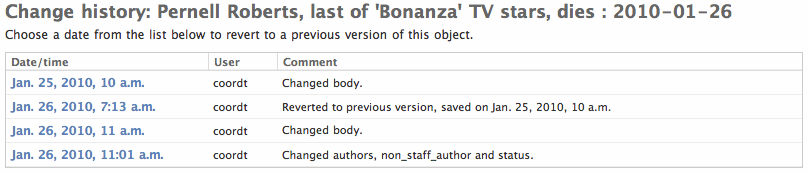
\includegraphics{history_list.png}

Each field of the story is shown with the values it contained in that version. It is not editable. You can leave the screen by clicking the browser's back arrow, or the ``Cancel'' button at the bottom of the screen.


\subsection{Reverting to a Previous Version}

Once you have opened up a previous version and want to revert back to it, click on the ``Revert to this version'' button.


\includegraphics{history_save_btn.png}


\subsection{Recovering a Deleted Story}

In the Stories listing, click on the ``Recover Deleted Story'' button in the upper-right corner of the page.


\includegraphics{recover_btn.png}

Then select a deleted story from the list by clicking on the timestamp.

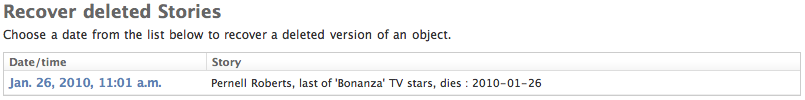
\includegraphics{recover_list.png}

The deleted story will open up as if you were editing it. Click the ``Save'' button to finish the recovery.


\chapter{Indices and tables}
\begin{itemize}
\item {} 
\emph{Index}

\item {} 
\emph{Module Index}

\item {} 
\emph{Search Page}

\end{itemize}


\renewcommand{\indexname}{Module Index}
\printmodindex
\renewcommand{\indexname}{Index}
\printindex
\end{document}
